\section{CHACHA 컴파일러}\label{sec:compiler}

CHACHA 컴파일러(CHACHA Compiler)는 snnTorch와 Brevitas로 QAT 학습된 SNN을 초소형 MCU용 정수 전용 코드로 lowering하는 모델 컴파일러다. 그림~\ref{fig:pipeline}은 전체 흐름을 보인다. PyTorch에서 학습된 모델로부터 정수 가중치와 스케일을 추출하고, 모든 스케일과 LIF 파라미터를 Q15 고정소수점으로 변환한 뒤, Conv+AvgPool 퓨전과 FC 퍼뮤트 패스를 거쳐 C 배열과 TFLite flatbuffer의 두 백엔드로 방출한다. 다만 CHACHA 컴파일러는 범용 중간 표현(IR) 기반 인프라가 아니라, QAT 학습 모델로부터 정수 파라미터를 추출$\cdot$변환하는 정수 전용 export 파이프라인과 C 배열$\cdot$TFLite flatbuffer 백엔드용 호스트 코드 생성기 2종으로 구성된 특화 컴파일러이다.

\begin{figure}[htbp]
\centering
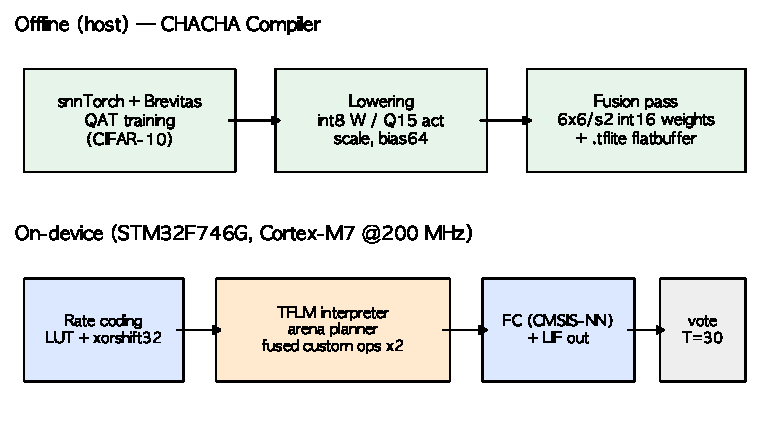
\includegraphics[width=0.9\linewidth]{figures/fig_pipeline.pdf}
\caption{CHACHA 컴파일러 전체 파이프라인. snnTorch+Brevitas QAT 학습 모델에서 정수 파라미터를 추출하고 Q15로 변환한 뒤, Conv+AvgPool 퓨전과 FC 퍼뮤트 패스를 거쳐 C 배열/TFLite flatbuffer 이중 백엔드로 방출한다.}
\label{fig:pipeline}
\end{figure}

\subsection{학습 파이프라인}\label{sec:compiler-train}

대상 모델은 LeNet-5급\cite{lecun1998gradient} SNN으로, Conv1($3\rightarrow32$, $5\times5$, 패딩 2)+AvgPool($2\times2$)+LIF1 $\rightarrow$ Conv2($32\rightarrow64$, $5\times5$, 패딩 2)+AvgPool+LIF2 $\rightarrow$ FC($4096\rightarrow10$)+LIF$_{out}$의 총 94,666 파라미터 구조다. CIFAR-10\cite{krizhevsky2009cifar}을 rate coding($T{=}30$)으로 인코딩해 입력하며, 전 레이어 공통으로 $\beta=0.9$, $\theta=1.0$을 사용한다. Conv/FC 레이어는 Brevitas\cite{brevitas2023}의 QuantConv2d/QuantLinear(\texttt{weight\_bit\_width}=8)로 구성하였고, 가중치 양자화기는 Brevitas 기본 설정을 사용하였다(per-tensor --- export 산출물의 스케일이 레이어당 스칼라 1개임을 확인). LIF는 snnTorch의 Leaky 뉴런(fast\_sigmoid 서러게이트 기울기)\cite{eshraghian2023training}이다. 학습 하이퍼파라미터와 학습 로그 정확도는 실험 재현 세부에 해당하므로 V장에서 실험 환경과 함께 기술한다. bias는 QAT 대상이 아니며 export 시 사후 양자화한다(다음 절).

\subsection{정수 전용 lowering}\label{sec:compiler-lowering}

제안 lowering의 원칙은 생성되는 C 코드에 float 타입과 리터럴을 일절 포함하지 않는 것이다. 가중치는 Brevitas의 \texttt{int\_weight()}로 int8 정수를 직접 추출하고, float 스케일 $s$는 모두 Q15 정수로 변환한다.
\begin{equation}
q = \mathrm{clip}\bigl(\mathrm{round}(s\cdot 2^{15}),\,-2^{15},\,2^{15}{-}1\bigr)
\label{eq:q15}
\end{equation}
예컨대 가중치 스케일은 conv1 $w_s{=}231$, conv2 $534$, FC $639$로, LIF 파라미터는 $\beta\rightarrow29{,}491(=\mathrm{round}(0.9\cdot2^{15}))$, $\theta\rightarrow32{,}767$(1.0의 포화값)로 방출된다. bias는 float 값을 $s_b=\max|b|/127$의 대칭 int8로 사후 양자화하고 Q15 스케일 $b_s$를 함께 방출한다.

정수 도메인 매핑은 다음과 같다. int8 가중치와 Q15 활성의 정수 누산을 $a=\sum_k w_k x_k$라 할 때, 비퓨전 기준 경로는
\begin{equation}
y_{q15} = \bigl\lfloor a\, w_s / 2^{15} \bigr\rfloor + b\, b_s
\label{eq:map-unfused}
\end{equation}
를 계산한 뒤 AvgPool이 /4 평균을 취한다(산술 시프트 절단과 풀링 반올림이 각각 발생). 퓨전 경로는 /4와 직전 층 스파이크 표현값 $s_{in}$의 보정을 하나의 실배율로 흡수한다.
\begin{equation}
M_f = \frac{w_s}{2^{15}} \cdot \frac{32767}{s_{in}} \cdot \frac{1}{4},\qquad
b_{64} = \mathrm{round}\!\left(\frac{b\, b_s}{M_f}\right)
\label{eq:mfused}
\end{equation}
출력은 $y=\mathrm{requant}(a_f+b_{64})$ 한 번으로 계산된다. 여기서 $a_f$는 퓨전 커널의 64비트 누산값이고, $M_f$는 \texttt{frexp}로 $M_f=q\cdot2^{e}$ ($q\in[0.5,1)$)로 분해되어 Q31 곱수 $m=\mathrm{round}(q\cdot2^{31})$과 시프트 $e$의 쌍으로 방출되며, 런타임은 CMSIS-NN의 64비트 requantize 루틴(\texttt{arm\_nn\_requantize\_s64})으로 이를 적용한다. 퓨전 경로는 반올림이 requantize 1회로 줄어든다. 두 경로의 수치 차이는 V장에서 분석한다(LIF1 스파이크의 0.75\%가 임계 근처에서 타이밍이 플립되나 최종 예측은 불변).

\subsection{Q15 활성 표현의 선택}\label{sec:compiler-q15}

활성값에 int8이 아닌 Q15(int16)를 사용하는 이유는 네 가지이다. 첫째, 감쇠 계수 $\beta=0.9$를 $29{,}491/32{,}768$로 표현할 수 있어 매 타임스텝 곱해지는 파라미터의 정밀도가 확보된다(int8이면 유효 정밀도가 부족하다). 둘째, 감산 리셋 후 잔여 막전위의 누적과 임계 비교에 충분한 동적 범위가 필요하다. 셋째, 스파이크를 0/32,767로 표현하면 Q15의 0/1.0에 대응한다. 넷째, Cortex-M7의 듀얼 16비트 SIMD(SMLALD, QADD16 등)가 s16 데이터를 자연스럽게 지원하므로 int8 대비 추가 비용이 없다.

\subsection{컴파일러 패스와 백엔드}\label{sec:compiler-passes}

\textbf{(1) Conv+AvgPool 퓨전 패스.} $5\times5$, 패딩 2 합성곱 뒤에 $2\times2$/스트라이드 2 평균 풀링이 이어지는 구성을 고려한다. 합성곱 출력은
\begin{equation}
c[m][n] = \sum_{u=0}^{4}\sum_{v=0}^{4} w_5[u][v]\; x[m{+}u{-}2][n{+}v{-}2]
\label{eq:conv5}
\end{equation}
이고(패딩 밖 $x$는 0), 풀링 출력은 $p[i][j]=\frac{1}{4}\sum_{dy,dx\in\{0,1\}} c[2i{+}dy][2j{+}dx]$이다. 식~(\ref{eq:conv5})를 대입하고 $a=u+dy$, $b=v+dx$로 치환하면
\begin{equation}
p[i][j] = \frac{1}{4}\sum_{a=0}^{5}\sum_{b=0}^{5} w_6[a][b]\; x[2i{+}a{-}2][2j{+}b{-}2]
\label{eq:fused6}
\end{equation}
\begin{equation}
w_6[a][b] = \sum_{dy,dx\in\{0,1\}} w_5[a{-}dy][b{-}dx]
\label{eq:w6}
\end{equation}
을 얻는다(첨자가 $[0,5)$ 범위를 벗어나는 항은 0). 즉 결과는 $2\times2$ 시프트된 $5\times5$ 커널 4개를 합친 $6\times6$ 커널을 스트라이드 2, 패딩 2로 적용한 합성곱과 같고, $1/4$은 식~(\ref{eq:mfused})의 requantize 배율 $M_f$에 흡수되므로 부동소수점 근사 없이 정수 수준에서 등가이다. bias는 네 풀링 위치에 동일하게 더해지므로 평균 후에도 변하지 않는다. 다만 $w_6$은 int8 값 4개의 합이라 $|w_6|\le508$이 되어 int8에 담기지 않으므로 int16으로 방출한다. 이것이 표준 CMSIS-NN s16 커널(int8 가중치 전용)을 사용할 수 없는 직접적 이유이며, IV장에서 커스텀 커널을 도입하는 근거가 된다. 연산량 감소와 커널 구현도 IV장에서 상술한다.

\textbf{(2) FC 퍼뮤트 패스.} 커널 출력(스파이크 텐서)은 NHWC 레이아웃인 반면 PyTorch의 FC 가중치는 CHW flatten 순서이므로, 빌드 타임에 $w'_{o,\,(8h+w)\cdot64+c}=w_{o,\,64c+8h+w}$($8\times8$ 공간, 64채널)로 재배열해 방출한다. 이로써 런타임 재배열이나 가중치의 RAM 사본이 필요 없다.

\textbf{(3) 이중 백엔드.} C 배열 백엔드는 퓨전 int16 가중치, int64 bias, (Q31 곱수, 시프트) 쌍을 const 배열(\texttt{snn\_weights\_fused.c/.h})로 방출하며 Flash에 상주시킨다. conv2 퓨전 가중치는 147,456B($\approx$147.5KB)로 SRAM(320KB)에 두기 어려워 Flash 상주가 전제된다. TFLite flatbuffer 백엔드는 커스텀 연산자를 포함한 TFLite 모델을 생성한다. 활성 텐서는 scale $1/2^{15}$, zero-point 0의 int16으로 Q15와 동일한 해석이고, 스파이크는 전 레이어 32,767로 표현한다(64비트 누산으로 오버플로가 없다 --- IV장). 퓨전 가중치 scale은 $w_s/(2^{15}\cdot4)$(평균 /4 흡수)를 CMSIS-NN 컨벤션에 따라 채널 수만큼 복제한 per-channel 배열로, bias는 입력 scale과 가중치 scale의 곱을 scale로 갖는 int64로 방출한다. 한편 C 배열 백엔드는 LIF1 출력 스파이크를 int32 누산 범위 내에서 정의된 표현인 16,384(Q14)로 나타내며, 그 보정 계수 $32767/16384$이 식~(\ref{eq:mfused})의 $M_f$에 흡수된다. 두 백엔드 모두 동일한 매핑식의 특수화이며, 생성물의 비트 정확성은 V장에서 검증한다.

현재 컴파일러가 지원하는 연산자는 본 그래프의 구성 요소(Conv, AvgPool, LIF, FC)이고, 실기기에서 검증된 모델은 본 논문의 LeNet-5급 SNN 1종이다.
